\documentclass{article}
\usepackage[left=0.85in, right=0.85in, top=0.5in, bottom=0.95in]{geometry}
\usepackage[T1]{fontenc}
\usepackage[utf8]{inputenc}
\usepackage[italian]{babel}
\usepackage{graphicx}
\usepackage{wrapfig2}
\usepackage{amsmath}
\usepackage{amssymb}
\usepackage{cases}
\usepackage{subcaption}
\usepackage{hyperref}
\hypersetup{
	colorlinks=true,
	linkcolor=blue,    
	urlcolor=blue,
	pdfpagemode=FullScreen,
}
\urlstyle{same}
\usepackage{changepage}
\usepackage{lastpage, epstopdf}
\usepackage{fancyhdr}
\usepackage{tcolorbox}
\usepackage{background}


%=======HEADER & FOOTER=======%
\def\lesson{Lesson Title}
%\def\outcome{\textbf{Learning Outcomes:} Outcomes go here. }

%\pagestyle{fancy}
%\fancyhf{}
%\renewcommand{\headrulewidth}{0pt}
%\renewcommand{\footrulewidth}{1.4pt}
%\lfoot{My Name $\diamond$ \the\year}
%\cfoot{Page \thepage/\pageref{LastPage}}
%\rfoot{\lesson}

%=======CORNELL STYLE FORMAT=======%
\SetBgScale{1}
\SetBgAngle{0}
\SetBgColor{black}
\SetBgContents{\rule{1pt}{0.899\paperheight}}
\SetBgHshift{-1.6in}
\SetBgVshift{-0.1in}

%=======CUSTOM BOXES=======%

\parindent 0ex

%=======BODY=======%
\begin{document}
	%\setcounterpageref{secnumdepth}{0}
	\section*{MECCANICA DEI SOLIDI: PARTE 1} %Date: \hrulefill}
%	\begin{tcolorbox}{\outcome}\end{tcolorbox}
	
	\begin{adjustwidth}{2in}{} 
		
%		\begin{wrapfigure}{l}0.25\textwidth}
%			\includegraphics[width=1\linewidth]{"Carica&Scarica/Scarica RC"}
%			\label{fig:RC}		
%		\end{wrapfigure}

{\Large \textbf{Richiami di geometria}} \mbox{} \newline
\begin{itemize}
\item Spazio vettoriale V \newline
		Contiene i vettori di partenza e quelli risultato della combinazione lineare.
	
\item Spazio Euclideo \newline
		Spazi vettoriali fisici tangibili formati da vettori a tre componenti. 
		
\item Base di spazio vettoriale \newline
		Insieme di vettori linearmente indipendenti tale che le loro combinazioni lineari diano tutti gli elementi di V. 
		
		Data la base $(e_1, e_2, e_3)$ si può definire un vettore di $R^3$ come:
		\[\vec{V} = V_1\vec{e}_1 + V_2\vec{e}_2 + V_3\vec{e}_3\]
		
\item Prodotto scalare 
		\[\vec{V} \cdot \vec{W} = V_1W_1 + V_2W_2 + V_3W_3 \]
		
\item Prodotto vettoriale 
		\[\vec{V} \times \vec{W} = V_1W_2\vec{e}_3-V_1W_3\vec{e}_2 -V_2W_1\vec{e}_3 + V_2W_3\vec{e}_1 + V_3W_1\vec{e}_2 - V_3W_2\vec{e}_1 \]
		Approccio pratico: 
\begin{itemize}
			\item Ogni termine è un vettore dato dal prodotto vettoriale di due vettori;
			\item $V_1W_2\vec{e}_3 = V_1\vec{e}_1 \times W_2\vec{e}_2 = V_1W_2(\vec{e}_1 \times \vec{e}_2)$
			\item $V_1\vec{e}_1 \times W_3\vec{e}_3 = V_1W_3(\vec{e}_1 \times \vec{e}_3) = - V_1W_3\vec{e}_2$
\end{itemize}
		Terna destrorsa: il 3° dito dà il risultato 
\begin{itemize}
			\item[(a)] Pollice 1° vettore
			\item[(b)] Indice 2° vettore 
			\item[(c)] Medio risultato
\end{itemize}
	
		Regola pratica 
		\[\underset{-}{\underleftarrow{ijk}}\underset{+}{\underrightarrow{ijk}}\]
		
		\[ \begin{aligned}
			i \times j & = k \\
			j \times k & = i \\
			k \times i & = j
		\end{aligned} \hspace{2cm} \begin{aligned}
		k \times j & = -i \\
		j \times i & = -k \\
		i \times k & = -j
	\end{aligned} \]
	
	Dunque per i versori degli assi $x,y,z$, rispettivamente $\hat{i}, \hat{j}, \hat{k}$, si ha: 
	\[
	\begin{cases}
		\hat{i}\times\hat{j}=\hat{k} \\
		\hat{j}\times\hat{k}=\hat{i} \\
		\hat{i}\times\hat{k}=-\hat{j} ~ oppure ~ \hat{k}\times\hat{i}=\hat{j}
	\end{cases}
	\]
		
\item Norma o modulo di $|| \vec{V} ||=\sqrt{V_{1}^2 + V_{2}^2 +V_{3}^2}$ \newline
\begin{figure}[H]
			\centering
						\includegraphics[width=0.2\textwidth]{"immagini/1.PARTE1_Pagina_03"}			
\end{figure}
\end{itemize}
		La base utilizzata sarà una base ortonormale destrogira $(e_{1},e_{2},e_{3})$ tale che:
		\[e_{1} \cdot e_{2} \times e_{3}= e_{1} \cdot e_{1}  =  1\]  
		
	In uno spazio di punti, presi due punti, questi definiscono un vettore:\newline 
	La posizione di un punto $P$ generico rispetto all'origine della terna o base è un vettore.
		\[P-O=\vec{V}\] 
		Si definisce quindi spazio affine euclideo $\xi$, se presi:
		\[(P,Q)\in \xi \Rightarrow \exists \vec{V}: \vec{V}=P-Q\]
		Ogni coppia di punti è legata da una relazione di tipo vettoriale. \newline
		Si può sempre definire una posizione relativa fra due punti appartenenti allo spazio euclideo. \newline
		

{\Large \textbf{Sistemi di forze}} \mbox{} \newline
Si definisce \textbf{corpo} un insieme aperto di punti all'interno dello spazio euclideo affine.\newline
un insieme A si dice aperto se contiene i punti di A: 
\[\forall x \in A ~ \exists ~ u_{x} : ~ \subset ~ \text{punti di A}\]
Ovvero se esiste un insieme o superficie $u_x$ che contiene i punti di A. \newline

Un corpo $\Omega$ si dice \textbf{rigido} se, per ogni configurazione spaziale del corpo:
\[\forall (P,Q) \in \Omega \Rightarrow \Vert(P-Q)\Vert=cost\]
La distanza relativa tra  i punti che lo compongono rimane costante. 

Un corpo rigido non si deforma ma si sposta. 

Si possono avere spostamenti differenti pur valendo la definizione di corpo rigido? Si, con una rotazione intorno ad un polo.

Le traslazioni sono campi di moto uniformi. \newline

Una \textbf{forza} è una qualunque causa che, se applicata ad un corpo, tende a modificarne lo stato di quiete, di moto o a causarne una deformazione. \newline
\begin{itemize}
	\item Forza Concentrata: rappresentata da un vettore $\vec{F}$ applicato, funzione della posizione e della velocità del punto, nonché del tempo.
	
	$F(t)$ è una forza impulsiva o tempo variabile;
	$F(\dot{x})$ può essere vista come una forza di resistenza, come quella dell'aria. 
	
	
	È rappresentato dalle coordinate $(\vec{F}, P)$ che indicano la forza in modulo, direzione e verso e il punto di applicazione $P$. \newline 
	\newpage
	\item Momento Polare: momento della forza  $\vec{F}$ rispetto al polo O, per un problema piano:
	\[
	\begin{split}
	\vec{M_{O}}(\vec{F}) & = (P-O)\times \vec{F} \\
	\Vert\vec{M_{O}}(\vec{F})\Vert & = \vert\vec{F}\vert ~ \vert(P-O)\vert ~ \sin\alpha = \vert\vec{F}\vert \cdot d
	\end{split}
	\]
	Il momento polare è una grandezza che dipende dal polo, il quale non è necessario appartenga al corpo.
	
	$d$ è proprio la distanza punto - retta. \newline 
	
	\item Coppia di forze: sistema di due forze $\vec{F}$ uguali e contrarie applicate ai due punti $P_{1}, P_{2}$.
	\begin{figure} [H]
		\centering
		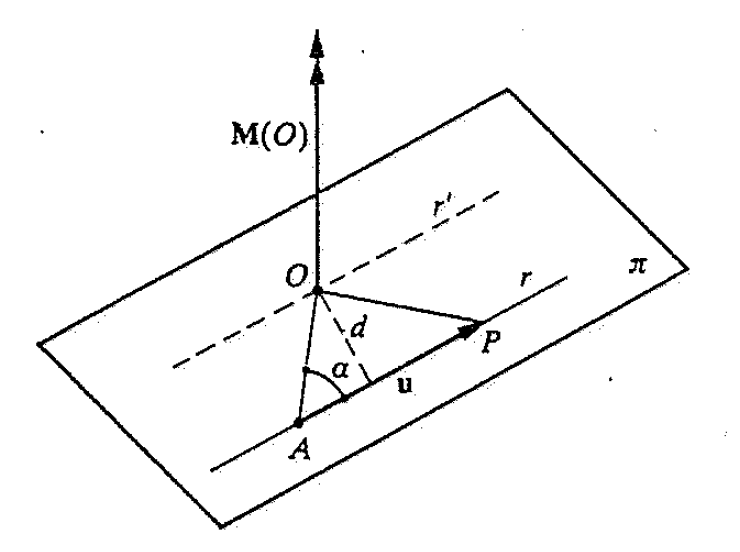
\includegraphics[scale=0.2]{immagini/image-012}
		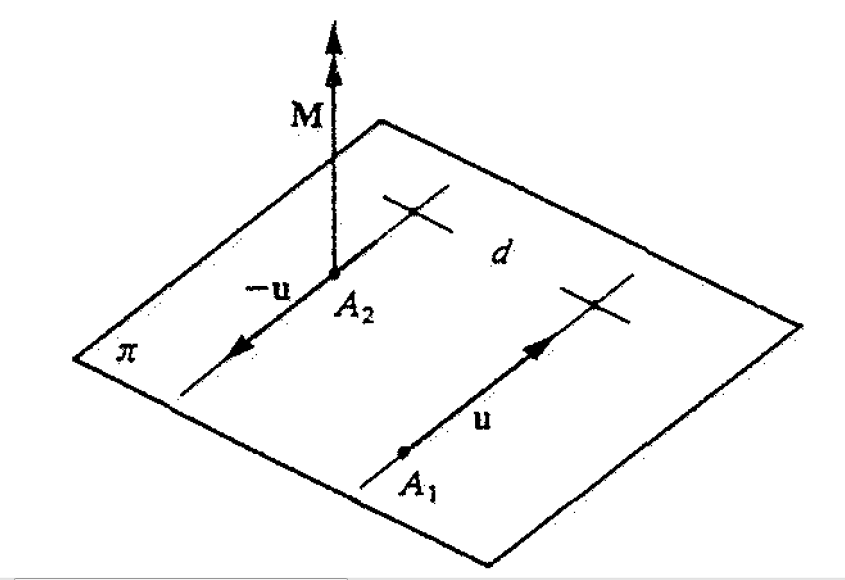
\includegraphics[scale=0.2]{immagini/image-013}
	\end{figure}
	
		\[
		\vec{M_{O}} = \overbrace{(P_{1}-O)\times \vec{F_{1}}}^\text{$M(\vec{F}_1)$} + \overbrace{(P_{2}-O)\times \vec{F_{2}}}^\text{$M(\vec{F}_2)$}
		\] 
		\[\vec{F}_1 = -\vec{F}_2\]
	\[
	\begin{split}
			\vec{M_{O}}	& = (P_{1}-O)\times \vec{F} - (P_{2}-O)\times \vec{F} =\\
		& = (P_{1}- O - P_{2} + O) \times \vec{F} = (P_{1} - P_{2})\times \vec{F} \\
		& = \underbrace{|P_1P_2|\vec{e}_1 \times F\vec{e}_1}_\text{$0$ componente lungo la forza} + \underbrace{|P_1P_2|\vec{e}_2 \times F\vec{e}_1}_\text{$d$ componente ortogonale}
	\end{split}
	\]
	\[\vert\vec{M_{O}}\vert = \vert\vec{F}\vert \cdot d\]
	
	NB: $\vec{(P-O)}$ è il vettore che punta verso P.
	
Una coppia di forze o un momento concentrato è null'altro che un vettore momento applicato: $(\vec{M}, Q)$. 
\end{itemize}
\newpage
Su un corpo rigido possono agire contemporaneamente forze e momenti concentrati. \newline
Si definisce sistema di forze l'insieme: 
\[ 
\begin{split}
S={(\vec{F_{i}}, P_{i}); (\vec{M_{j}}, Q_{j})}\\ i=1\dots n; j=1\dots m
\end{split}
\]
Per un sistema di forze si definiscono \textbf{Risultante} e \textbf{Momento Risultante} come i descrittori statici di un dominio, ovvero le informazioni sintetiche attribuibili ad un sistema di forze: 
\begin{itemize}
	\item Risultante: Somma vettoriale dei vettori forza.
	\[
	\vec{R} = \sum_{i=1}^{n} \vec{F_{i}}
	\]
\item Momento Risultante: somma dei momenti generati dalle forze (primo termine) e dei momenti concentrati (secondo termine) rispetto ad un polo arbitrario O.
	\[
	\vec{M_{O}} = \sum_{i=1}^{n} (P_{i}-O)\times \vec{F_{i}} + \sum_{j=1}^{m} \vec{M_{j}}
	\]	
	\end{itemize}
I descrittori statici sono elementi che descrivono lo stato di applicazione delle forze sul corpo in modo più sintetico che considerare ogni contributo. \newline 


{\Large \textbf{Proprietà dei descrittori statici}} 	\mbox{} \newline
\begin{enumerate}
\item $\vec{M_{O}} ~ e ~ \vec{R}$ non dipendono dai punti Q di applicazione del momento in quanto banalmente non appaiono nelle loro definizioni.
\item  $\vec{M_{O}} ~ e ~ \vec{R}$ non variano spostando una forza lungo la sua retta d'azione.
\begin{figure}[H]
	\centering
	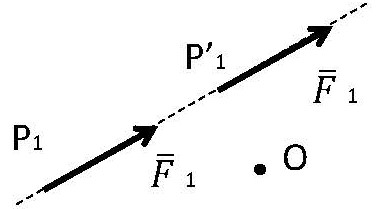
\includegraphics[width=0.2\linewidth]{immagini/1.PARTE1_Pagina_07}
\end{figure}

	\[
	\vec{M_{O}} = (P_{1}-O)\times \vec{F_{1}} + \dots + (P_{n}-O)\times \vec{F_{n}} + \sum_{j=1}^{m} \vec{M_{j}}
	\]
	Traslo a questo punto $\vec{F_{1}}$ lungo la sua direzione:
	
	\[ 
	\vec{M'_{O}} = (P'_{1}-O)\times \vec{F_{1}} + \dots + (P_{n}-O)\times \vec{F_{n}} + \sum_{j=1}^{m} \vec{M_{j}}
	\]
	ove $(P'_{1}-O) = (P'_{1} - P_{1} + P_{1} - O)$ e dunque:
	
		\[ 
	\vec{M'_{O}} = (P'_{1}-P_{1})\times \vec{F_{1}} + (P_{1}-O)\times \vec{F_{1}} \dots + (P_{n}-O)\times \vec{F_{n}} + \sum_{j=1}^{m} \vec{M_{j}}
	\]
ma $ (P'_{1}-P_{1}) \times \vec{F_{1}} = 0 : (P'_{1}-P_{1})\parallel\vec{F_{1}}$. \newline
Si giunge così a: 
	\[ 
\vec{M'_{O}} = (P_{1}-O)\times \vec{F_{1}} \dots + (P_{n}-O)\times \vec{F_{n}} + \sum_{j=1}^{m} \vec{M_{j}} = \vec{M_{O}}
\]
\[ \vec{M'_{O}} = \vec{M_{O}} ~~~~ \blacksquare \]

\item Legge di variazione del polo. \newline
Il momento di un sistema di forze calcolato rispetto ad un polo A arbitrario è legato al momento polare in O come: 
\[ 
\vec{M_{A}}=\vec{M_{O}} + (O-A)\times \vec{R}
\]
Dove $(O-A)$ è la posizione del vecchio polo rispetto al nuovo.
\[ 
\vec{M_{A}}= \sum_{i=1}(P_{i} - A) \times \vec{F_{i}} + \sum_{j=1}\vec{M_{j}}
\]
Essendo $(P_{i} - A)=(P_{i}-O+O-A)$ allora: 
\[ 
\vec{M_{A}}= \sum_{i=1}(O - A) \times \vec{F_{i}} + \sum_{i=1}(P_{i} - O) \times \vec{F_{i}} + \sum_{j=1}\vec{M_{j}}
\]

Ma:
\[ 
\sum_{i=1}(P_{i} - O) \times \vec{F_{i}} + \sum_{j=1}\vec{M_{j}} = \vec{M_{O}}
\] 

E quindi: 

\[ 
\vec{M_{A}}= \sum_{i=1}(O - A) \times \vec{F_{i}} + \vec{M_{O}} = (O - A) \times \sum_{i=1}\vec{F_{i}} + \vec{M_{O}} 
\]

\[ 
\vec{M_{A}} = (O - A) \times \vec{R} + \vec{M_{O}} ~~~~ 
\blacksquare\]

\item Equivalenza dei sistemi di forze \newline
A cosa serve ricondurre un sistema di forze a 2 descrittori statici? Definisco un criterio di equivalente tra sistemi di forze che risponda alla domanda: hanno due sistemi di forze lo stesso effetto? 

Due sistemi di forze S ed S' sono equivalenti se: 
 \begin{enumerate}
 	\item $\vec{R}=\vec{R'}$
 	\item $\exists O ~ polo : \vec{M_{O}}=\vec{M'_{O}}$
 	\end{enumerate}
 
Corollario: se S ed S' sono equivalenti, allora $\vec{M_{O}}=\vec{M'_{O}} ~ \forall ~ polo$
 
 \[ 
 \vec{M_{A}}= (O - A) \times \vec{R} + \vec{M_{O}}  
 \]
 \[ 
 \vec{M'_{A}}= (O - A) \times \vec{R'} + \vec{M'_{O}}  
 \]
 Essendo, per definizione di equivalenza $\vec{R}=\vec{R'}$, $\vec{M_{O}}=\vec{M'_{O}}$, si ha infine: 
 
 \[ 
 \vec{M_{A}}=\vec{M'_{A}}
 \]
 \textit{Esempio A}: si ponga il sistema di forze  in (1) e ci si chieda se è equivalente a quello in (2): 
 \begin{figure}[H]
 	\centering
 	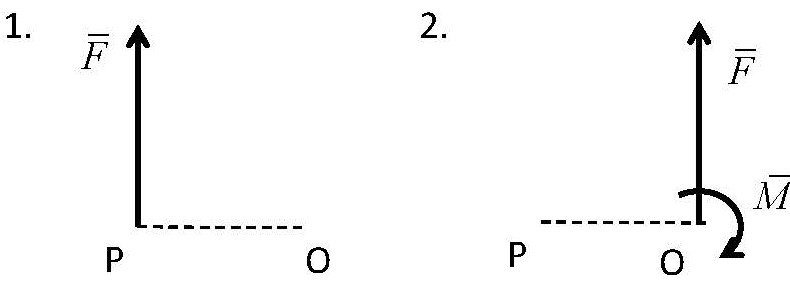
\includegraphics[width=0.25\linewidth]{immagini/1.PARTE1_Pagina_10}
 \end{figure}
 \[ 
 \begin{cases}
 	\vec{R_{1}}=\vec{R_{2}}=\vec{F} \\
 	\vert\vec{M^1_{O}}\vert = \vert\vec{F}\vert ~ d \\
 	\vert\vec{M^2_{O}}\vert = \vert\vec{M}\vert
 \end{cases}
 \]
In (2) la retta d'azione di F passa per il polo O: $M_F=0$
E i due sistemi si diranno equivalenti se il momento $M$ di trasporto $\vert\vec{M}\vert$ è:
\[ 
\vert\vec{M}\vert=\vert\vec{F}\vert \cdot d
\]
\newpage
\item Teorema del trasporto \newline
Posso spostare una forza perpendicolarmente alla direzione mantenendo il sistema equivalente, aggiungendo un momento di trasporto pari al momento dato dalla forza posizionato nel punto di partenza, rispetto al punto di arrivo.

\textit{Esempio B}: I 3 sistemi di forze sono equivalenti?
\begin{figure}[H]
	\centering
	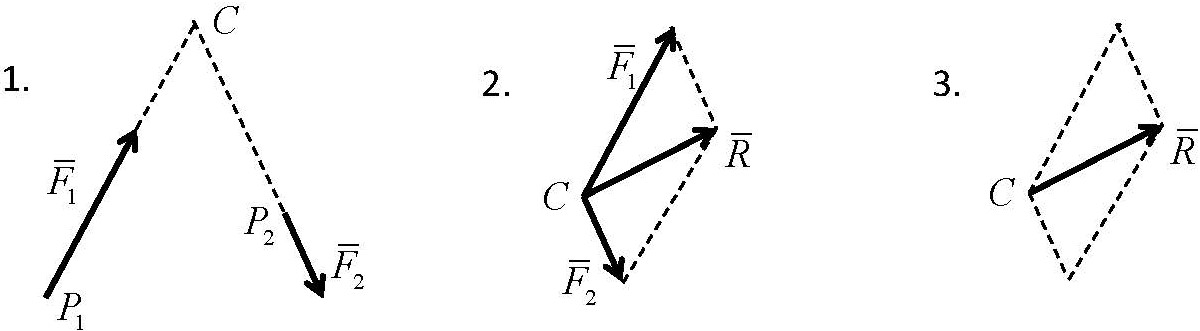
\includegraphics[width=0.25\linewidth]{immagini/1.PARTE1_Pagina_11}
\end{figure}
Dove in (3) la risultante è stata proprio definita così a priori. 
\[ 
\begin{split}
\vec{R_{1}}= & \vec{R_{2}}=\vec{R_{3}} = \vec{F_{1}}+\vec{F_{2}}\\
\vec{M'_{O}}= & (P_{1}- O) \times \vec{F_{1}} + (P_{2}- O) \times \vec{F_{2}}
\end{split}
\]
\[\vec{M}_0^2 = (C-O) \times \vec{F}_1 + (C-O) \times \vec{F}_2 \]
È cambiato il punto di applicazione, questo giace su entrambe le rette d'azione delle forze. Il momento risultante cambia per traslazione di forze lungo la retta d'azione? No per il punto n.2.

Traslando perciò lungo la retta d'azione: 
\[ 
\vec{M^1_{O}}= (C - O) \times \vec{F_{1}} + (C- O) \times \vec{F_{2}} = \vec{M^2_{O}}= (C - O) \times (\vec{F_{1}} + \vec{F_{2}}) = (C- O) \times \vec{R} = \vec{M^3_{O}}
\]
Attravero il sistema (2) si è così dimostrata l'equivalenza tra il sistema (1) e (3).

Un sistema di due forze con rette d'azione concorrenti in più punti è equivalente al sistema di una forza uguale alla risultante, applicata nel punto di incontro delle rette d'azione, punto proprio. \newline

\textit{Esempio C}: dov'è applicata la risultante?
\begin{figure}[H]
	\centering
	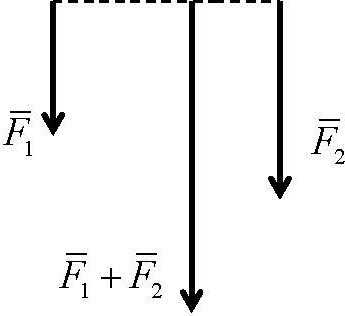
\includegraphics[width=0.25\linewidth]{immagini/1.PARTE1_Pagina_12}
\end{figure}
La risultante $F_1 + F_2$ è applicata in modo tale da verificare l'equivalenza tra i momenti:
 \[ 
\begin{cases}
	\vec{R} = \vec{F_{1}} + \vec{f_{2}} \\
	\vert\vec{M_{O}}\vert = \vert\vec{F_{1}}\vert ~ d_{1}  + \vert\vec{F_{2}}\vert ~ d_{2}\\
	\vert\vec{M' _{O}}\vert = \vert\vec{F_{1}} + \vec{F_{2}}\vert ~ d
\end{cases} \Rightarrow \vert\vec{M_{O}}\vert = \vert\vec{M' _{O}}\vert \Leftrightarrow d = \dfrac{d_{1}F_{1} + d_{2}F_{2}}{F_{1}+F_{2}}
\]
\newpage
\item Equilibrio di un sistema di forze applicate su un corpo rigido.\newline
Un corpo si dice in equilibrio se su esso è applicato un sistema di forze in equilibrio. \newline
Un sistema di forze si dice in equilibrio se e solo se è equivalente a zero. 
\[ 
\begin{cases}
	\vec{R} = 0 ~ Equilibrio ~ a ~ Traslazione \\
	\exists ~ O : \vec{M_{O}} = 0 ~ Equilibrio ~ a ~ Rotazione \\
	\end{cases}
\]

Una volta dimostrato il sistema essere in equilibrio allora vale la condizione necessaria e sufficiente: 
\[ 
S ~ è ~ in ~ equilibrio \Leftrightarrow \vec{M_{A}} = 0 ~ \forall A
\]
A cui si aggiunge il corollario: Se il momento risultante è nullo per almeno due poli, allora il sistema è in equilibrio.
Siano $ O_{1}, O_{2}, O_{3}$ tre punti non allineati e per ipotesi si abbia $\vec{M_{O1}} = \vec{M_{O2}} = \vec{M_{O3}}$, per la legge di variazione del polo si può scrivere:
\[ 
\begin{cases}
	\vec{M_{O2}} = \vec{M_{O1}} + (O_{1} - O_{2})\times \vec{R} \\
	\vec{M_{O3}} = \vec{M_{O1}} + (O_{1} - O_{3})\times \vec{R}
	\end{cases} \Rightarrow \begin{cases}
	(O_{1} - O_{2})\times \vec{R} = 0 \\
	(O_{1} - O_{3})\times \vec{R} = 0
	\end{cases}  \Rightarrow \begin{cases}
		(O_{1} - O_{2}) \parallel \vec{R}  \\
	(O_{1} - O_{3})\parallel \vec{R} 
	\end{cases}
\]
E ciò diviene possibile se: 
\begin{enumerate}
	\item $(O_{1} - O_{2}) \parallel (O_{1} - O_{3})$; 
	\item $\vec{R} = 0$
\end{enumerate}
Mentre la prima è negata per ipotesi, la seconda conferma il fatto che il sistema S è in equilibrio. $\blacksquare$
\newpage
\begin{itemize}
\item[$\Rightarrow$] Due forze in equilibrio

Un sistema di due forze è in equilibrio se e solo se la risultante è nulla, le forze sono uguali e contrarie ed agiscono sulla stessa retta d'azione. \newline
\begin{figure}[H]
	\centering
	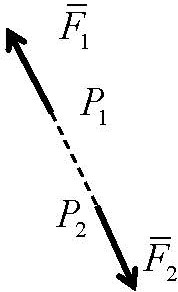
\includegraphics[width=0.2\linewidth]{immagini/1.PARTE1_Pagina_14}
\end{figure}

Se il sistema è in equilibrio allora la risultante delle forze ed il momento devono essere nulle: $\vec{R} = \vec{M_{O}} = 0$. 

Poste essere le due forze $\vec{F_{1}} = - \vec{F_{2}}$ (la somma deve essere nulla), si può scrivere:
\[ 
\begin{split}
	\vec{M_{O}} & = (P_{1}-O)\times \vec{F_{1}} + (P_{2} -O) \times \vec{F_{2}} =\\
	& = (P_{1} - O - P_{2} - O) \times \vec{F_{1}} = \\
	\vec{M_{O}} & = (P_{1} - P_{2} ) \times \vec{F_{1}} \underbrace{= 0}_\text{Imponendo l' equilibrio}
\end{split}
	\]
	$(P_1 - P_2)$ è la congiungente dei punti di applicazione delle forze ed è parallela ad $F_1$:
	\[(P_1 - P_2) \parallel F_1\]
	Ma $F_1 = -F_2$ e dunque:
	\[
	(P_{1} - P_{2})  \parallel \vec{F_{2}} \parallel \vec{F_{1}} \blacksquare
\]
Due vettori che sono paralleli e condividono un punto comune sono collineari. \newline

\item[$\Rightarrow$] Tre forze in equilibrio

Un sistema di tre forze è in equilibrio se e solo se la risultante è nulla e le forze sono complanari e con rette d'azione concorrenti tra loro [= in pratica non sono parallele tra loro]. \newline
\begin{figure}[H]
	\centering
	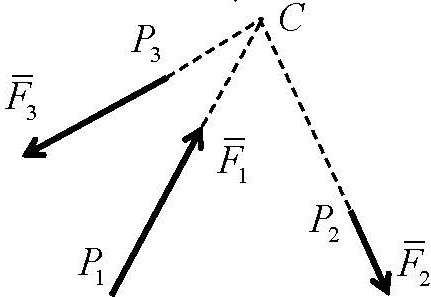
\includegraphics[width=0.2\linewidth]{immagini/1.PARTE1_Pagina_15}
	\caption{}
	\label{fig:}
\end{figure}

Se il sistema è in equilibrio allora la risultante delle forze ed il momento devono essere nulle: $\vec{R} = \vec{M_{O}} = 0$.
\[ 
\begin{split}
	\vec{M_{P_{1}}} & = (P_{1}-P_{1})\times \vec{F_{1}} + (P_{2} -P_{1}) \times \vec{F_{2}} + (P_{3}- P_{1}) \times \vec{F_{3}} \underbrace{= 0}_\text{Imponendo l' equilibrio}\\
	& = (P_{2} -P_{1}) \times \vec{F_{2}} + (P_{3}- P_{1}) \times \vec{F_{3}} = 0 \\
	& = (P_{2} -P_{1}) \times \vec{F_{2}} \cdot (P_{3}- P_{1}) + (P_{3}- P_{1}) \times \vec{F_{3}} \cdot (P_{3}- P_{1}) = 0 \\
\end{split}
\]
Moltiplicando perciò per lo stesso termine $(P_{3}- P_{1})$ ci si accorge che la quantità: 
\[ (P_{3}- P_{1}) \times \vec{F_{3}} \cdot (P_{3}- P_{1}) =0 \]
Per le proprietà del prodotto vettoriale. 

Rimarrà dunque:
\[\vec{M_{P_{1}}}  = (P_{2} -P_{1}) \times \vec{F_{2}} \cdot (P_{3}- P_{1})\]

Si nota allora che:
\[(P_3 - P_1) \perp [(P_2 - P_1) \times \vec{F}_2]\]
$P_3$ dev'essere perciò sul piano già contenente $P_1$ e $P_2$, le forze devono essere complanari.

Ci si accorge inoltre che $\vec{F_{2}}$ appartiene al piano contenente i punti di applicazione, come anche  $\vec{F_{2}}$, e quindi, rispetto ai poli  $P_{3}, P_{2}$ varrà equivalentemente: 
\[ 
(P_{3} -P_{1}) \times \vec{F_{3}} \cdot (P_{2}- P_{1}) = 0
\]
Ipotizzando poi che $ \vec{F_{1}}, \vec{F_{3}}$ concorrano in un punto C, allora il momento rispetto a tale polo di $F_2$ sarà: 
\[ 
(P_{2} - C) \times \vec{F_{2}} \equiv 0
\]
Per l'equilibrio ora imposto, allora: 
\[ 
(P_{2} - C) \parallel \vec{F_{2}} 
\]
E le tre rette d'azione concorrono nello stesso punto. $\blacksquare$ \newline
Un sistema in equilibrio può essere rappresentato da un poligono di lati pari al valore delle forze e versi uguali a quelli dei vettori posti in maniera tale che si inseguono. 
\begin{figure}[H]
	\centering
	\includegraphics[width=0.1\linewidth]{"immagini/1.PARTE1_Pagina_16 (2)"}
\end{figure}
\newpage
\item[$\Rightarrow$] In caso di rette d'azione parallele, posso avere equilibrio anche se le forze non sono concorrenti in un punto, ma queste devono essere complanari. 
\begin{figure}[H]
	\centering
	\includegraphics[width=0.2\linewidth]{"immagini/1.PARTE1_Pagina_16 (3)"}
\end{figure}
\[ 
\vec{R} = 0
\begin{split}
\vec{M_{P_{1}}} & = (P_{1}-P_{1})\times \vec{F_{1}} + (P_{2} -P_{1}) \times \vec{F_{2}} + (P_{3}- P_{1}) \times \vec{F_{3}} = 0\\
& = (P_{2} -P_{1}) \times \vec{F_{2}} + (P_{3}- P_{1}) \times \vec{F_{3}} = 0 \\
\end{split}
\]
\[
\vec{F_{2}} \parallel \vec{F_{3}} \Rightarrow ~ Complanari 
\]
\[
\vec{F_{1}} = -(\vec{F_{2}} + \vec{F_{3}}) \Rightarrow ~ Complanari ~~~~ \blacksquare
\]
\item[$\Rightarrow$] Un sistema si dice piano se può essere rappresentato su di un piano $\Pi$. 
\[ 
\exists~\pi : \begin{cases}
	P_{i} \in~\pi \Rightarrow F_{i} \parallel \pi, i = 1 \dots n \\
	Q_{j} \in~\pi \Rightarrow M_{j} \perp \pi, j = 1 \dots m \\
\end{cases}
\]
Ovvero, le forse applicate in punti del piano sono parallele al piano, mentre i momenti sono perpendicolari al piano. \newline
Le condizioni di equilibrio di un sistema di forze sono le equazioni cardinali della statica, che in questo caso divengono: 
\[ 
\begin{cases}
\vec{R} = 0 \\
\vec{M} = 0
\end{cases}
\]
Diventano un sistema di tre equazioni scalari: 
\[ 
\begin{cases}
	R_{x} = 0 \\
	R_{y} = 0
	M = 0
\end{cases}
\]
I moti possibili divengono  così 2 Traslazioni nel piano, lungo $x$ ed $y$ e una rotazione intorno all'asse $z$.

Ad un sistema piano si associano problemi piani. 

 


\end{itemize}
\end{enumerate}
\newpage
Quando si comincia a parlare di possibilità di moto di un corpo si introduce la
{\Large \textbf{Cinematica del corpo rigido}} \mbox{} \newline
Si ha un moto di Traslazione Pura quando i vettori rappresentativi la velocità di ciascun punto del corpo risultano essere tutti costanti, ovvero ad ogni punto appartenente al corpo si può associare il medesimo vettore velocità:
\[ \forall~P~\in~\Omega : \vec{v}=cost\]
Una Rotazione Rigida intorno ad un punto fisso è caratterizzata da una velocità angolare $\omega$ che può avere una componente per ogni asse nella base principale: 
\[ \vec{\omega} = (\omega_{1}, \omega_{2}, \omega_{3})\]
La velocità di un punto è data da: 
\[ \vec{v_{P}} = \vec{\omega} \times (P-O)
\]
E può essere espressa in forma matriciale in cui la matrice $[\omega]$ è antisimmetrica:
\[ 
\omega_{ij} = -\omega_{ji}
\]
\[
\omega = \left[\begin{array}{ccc}
	0 & -\omega_{3} & \omega_{2} \\
	\omega_{3} & 0 & -\omega_{1} \\
	-\omega_{2} & \omega{1} & 0
\end{array}\right]
\]

Il Moto Vario sarà dunque descritto da una traslazione piana e da una rotazione rigida, per cui: 
\[ \vec{v_{P}} = \vec{v_{0}} + \vec{\omega} \times (P-O)\]
\textbf{Spostamenti virtuali} \mbox{} \newline
Rappresentano l'atto di moto che quel corpo compirebbe in un $dt$ data quella specifica distribuzione di velocità.

Un corpo rigido sottoposto ad un generico campo di velocità in un infinitesimo intervallo temporale, compirà un altrettanto infinitesimo spostamento dato da:
\[
ds_{P} = \vec{v_{P}}dt + \vec{\omega}dt \times (P-O) = d\vec{s_{0}} + d\varphi \times (P-O)
\]
Dove $\omega$ e $\phi$ sono rispettivamente la velocità angolare e il relativo spostamento angolare associato che descrivono la rotazione infinitesima. \newline

Integrando così gli spostamenti virtuali infinitesimi definisco univocamente il campo di spostamenti virtuale come: 
\[
\vec{s}(P) = \vec{s_{0}} + \varphi \times (P-O)
\]
La ricostruzione degli angoli $\phi$ secondo gli assi cartesiani è però sensibile all'ordine di ricostruzione, si definiscono così gli \newline
 \textbf{Angoli di Eulero e la Matrice di Rotazione} \mbox{} \newline
 Oltre a definire gli assi cartesiani è necessario definire l'ordine col quale si ricostruiscono gli angoli.
  
Si vuole determinare le caratteristiche di variazione di configurazione del corpo rigido in moto facendo riferimento a soli parametri geometrici. \newline
\begin{figure}[H]
	\centering
	\includegraphics[width=0.5\linewidth]{"immagini/1.PARTE1_Pagina_19"}
\end{figure}
considerando un corpo libero di ruotare attorno ad un punto O fisso, la terna di riferimento inerziale fissa $(e_{1},e_{2},e_{3})$ e quella solidale al corpo $(u_{1},u_{2},u_{3})$ sono inizialmente coincidenti.\newline

\newpage
Dopo la rotazione si possono individuare gli angoli $\Psi, \varphi, \theta$ detti Angoli di Eulero, formatisi tra le terne ai quali si da il nome di: 
\begin{itemize}
	\item $\varphi$ Angolo di Precessione formato da $e_{1}$ e la proiezione di $u_{1}$ sul piano $e_{1}e_{2}$; 
	\item $\Psi$ Angolo di Rotazione Propria tra $u_{1}$ e il piano $e_{1}e_{2}$;
	\item $\theta$ Angolo di Nutazione tra $u_{3}$ ed $e_{3}$.
\end{itemize}
\begin{figure}[H]
	\centering
	\includegraphics[width=0.25\linewidth]{"immagini/1.PARTE1_Pagina_20"}
\end{figure}
Questi angoli così definiti danno luogo alla matrice Q. 

Il nuovo vettore posizione si ottiene per trasformazione lineare del precedete: 
\[ \underbrace{(P'-O)}_\text{Posizione finale} = [Q]\underbrace{(P-O)}_\text{Posizione iniziale}\]
Con $ [Q]=Q(\Psi, \varphi, \theta)$ matrice di rotazione, ortogonale. \newline
Si ricordi brevemente che una matrice ortogonale è caratterizzata dalle seguenti proprietà: 
\[ \begin{cases}
	det[Q] = 1\\
	[Q]^{-1} = [Q]^{-T} \Rightarrow [Q][Q]^{T} = [Q]^{T}[Q]=[I]
\end{cases}
\]
Si restringa il problema ad una rotazione piana considerando una rotazione rigida intorno al solo asse $e_{3}$:
\[ 
(P-O)=\left[\begin{array}{c}
	x_{P} \\
	0 \\
	0
\end{array}\right] \in \vec{e}_1; \hspace{1cm} 
(R-O)=\left[\begin{array}{c}
	0 \\
	y_{R} \\
	0
\end{array}\right] \in \vec{e}_2
\]
Dove sono P ed R a seguito di una rotazione piana? Dove sono P' ed R'?
\begin{figure}[H]
	\centering
	\includegraphics[width=0.25\linewidth]{"immagini/1.PARTE1_Pagina_21"}
\end{figure}
\[ 
(P'-O) = \left[\begin{array}{c}
	x_{P}\cos(\varphi) \\
	x_{P}\sin(\varphi) \\
	0
\end{array}\right]; \hspace{1cm} 
(R'-O) = \left[\begin{array}{c}
	-y_{R}\sin(\varphi) \\
	y_{R}\cos(\varphi) \\
	0
\end{array}\right] 
\]
\[
\begin{cases}
	(P'-O) = [Q](P-O)\\
	(R'-O) = [Q](R-O)
\end{cases}
\]
\newpage
E dunque in un moto piano la matrice di rotazione sarà: 

\[
Q = \left[\begin{array}{ccc}
	\cos(\varphi) & -\sin(\varphi) & 0 \\
	\sin(\varphi) & \cos(\varphi) & 0 \\
	0 & 0 & 1
\end{array}
\right]
\]
Dipendente solamente dall'angolo di precessione $\varphi$. \newline

In condizione di traslazione pura, lo spostamento legato ad esso sarà: 
\[\vec{s}_P = (P' - P) = cost ~ \forall P\]
In generale, per un corpo che subisce traslazione e rotazione posso immaginare:
\begin{enumerate}
	\item Una traslazione da P a P' 
	\item Una rotazione da P' a P" 
\end{enumerate}
\begin{figure}[H]
	\centering
	\includegraphics[width=0.3\linewidth]{"immagini/1.PARTE1_Pagina_22"}
\end{figure}
Perciò lo spostamento finale sarà dato da: 
\begin{enumerate}
	\item[2.] Rotazione
	\[(P''-O') = [Q](P'-O')\]
	\item[1.] Traslazione
	\[(P'-O') = (P-O)\]
\end{enumerate}
Ottenendo infine:
\[(P''-O')=[Q](P-O)\]
Ciò che interessa però è lo spostamento di P identificato da $P'' - P$, tale spostamento ci si accorge essere identificato da una somma di tre vettori ottenuta notando che:
\[ (P-O) + (P'' - P) = (O' - O) + (P'' - O') \]
E dunque:
\[\vec{s}_P = P'' - P = \left\lbrace (P'' - O') + (O' - O) - (P-O)\right\rbrace  \]
Sostituendo i termini ora noti:
\[\vec{s}_P = \left\lbrace [Q](P-O) + \vec{s}_0 - (P-O)\right\rbrace  \]
\[\vec{s}_P = \vec{s}_0 + ([Q] - [I])(P-O)  \]
Ottenendo così una formula generale del campo di spostamenti di un corpo rigido. \newline

Ora, ricordando che per un poto piano vale: 
\[
Q = \left[\begin{array}{ccc}
	\cos(\varphi) & -\sin(\varphi) & 0 \\
	\sin(\varphi) & \cos(\varphi) & 0 \\
	0 & 0 & 1
\end{array}
\right]
\]

Allora la matrice $[Q-I]$ sarà:
\[
Q -I = \left[\begin{array}{ccc}
	\cos(\varphi)-1 & -\sin(\varphi) & 0 \\
	\sin(\varphi) & \cos(\varphi)-1 & 0 \\
	0 & 0 & 1-1
\end{array}
\right]
\]
In caso di piccole variazioni si può porre $\cos(\varphi) \approx 1; \sin(\varphi) \approx \varphi$ e dunque:
\[
Q -I = \left[\begin{array}{ccc}
	0 & -\varphi & 0 \\
	\varphi & 0 & 0 \\
	0 & 0 & 0
\end{array}
\right]
\]
Ottenendo una matrice antisimmetrica proprio come la matrice delle velocità $[\omega]$.\newline

Per un corpo libero nello spazio si hanno garantite 3 possibilità di traslazione e 3 possibilità di rotazione, perciò un punto appartenente ad un corpo nello spazio gode di 6 gradi di libertà. Nel caso di problema piano i gradi di libertà si ridurranno a 3. \newline

Si definisca $\vec{\Phi}$ il vettore degli angoli di moto contenente i 3 atti di rotazione, allora banalmente per un moto piano si avrà:
\[\vec{\Phi} = \left\lbrace \begin{array}{c}
	0 \\
	0 \\
	\varphi
\end{array} \right\rbrace \]
Allora si può riscrivere: 
\[([Q] - [I])(P-O) = ([Q] - [I])\vec{r} = \vec{\Phi} \times \vec{r} \]
\[ ([Q] - [I])\vec{r} = \left[\begin{array}{ccc}
	0 & -\varphi & 0 \\
	\varphi & 0 & 0 \\
	0 & 0 & 0
\end{array}
\right] \left\lbrace \begin{array}{c}
	x \\
	y \\
	z
\end{array} \right\rbrace = \left[ \begin{array}{c}
0 -\varphi y + 0 \\
\varphi x +0 +0  \\
0
\end{array} \right] = \left[ \begin{array}{c}
-\varphi y \\
\varphi x   \\
0
\end{array} \right] \]

\[\vec{\Phi} \times \vec{r} =  \left\lbrace \begin{array}{c}
	0 \\
	0 \\
	\varphi
\end{array} \right\rbrace \times \left\lbrace \begin{array}{c}
x \\
y \\
z
\end{array} \right\rbrace = \left|  \begin{array}{ccc}
\hat{i} & \hat{j} & \hat{k} \\
0 & 0 & \varphi \\
x & y & z
\end{array} \right|  = \hat{i}(-\varphi y) - \hat{j}(-\varphi x) + \hat{k}\cdot 0 = \left[ \begin{array}{c}
-\varphi y \\
\varphi x   \\
0
\end{array} \right]_\blacksquare \]

Per un generico campo di spostamenti associato al moto di un corpo rigido si può dunque scrivere:
\[\vec{s}_P = \vec{s}_0 + \vec{\Phi} \times (P-O)\]

I vettori $ \vec{s}_0,\vec{\Phi}$ si dicono descrittori cinematici, necessari questi a trovare lo spostamento incognito di P, conoscere i descrittori cinematici implica la conoscenza della cinematica del corpo (o punto), ovvero come si sposta.

\newpage


{\Large \textbf{Lavoro Virtuale}} \mbox{} \newline
Si consideri un corpo rigido a cui sia associato un sistema di forze, a questi si possono associare due descrittori statici e due descrittori cinematici: 
\[ (\vec{M_{O}}; \vec{R}), (\vec{s_{0}}; \vec{\Phi})\]
I descrittori cinematici possono essere completamente indipendenti da quelli statici, cioè si possono associare al corpo spostamenti non dovuti al sistema di forze su esso applicato. \newline
il Lavoro Virtuale di un sistema di forze è il lavoro che questo sistema compirebbe se fosse sottoposto a spostamenti virtuali associati al corpo - descritti dai descrittori cinematici -, indipendentemente dal sistema di forze su esso applicato.
\begin{equation}
	L_{V} = \sum_{i=1}^{n}(\vec{F_{i}} \cdot \vec{s_{P_{i}}}) + \sum_{j=1}^{m}(\vec{M_{j}} \cdot \vec{\Phi})
\end{equation} 
\[ 
\vec{s_{P_{i}}} = \vec{s_{0}} + \vec{\Phi} \times (P_{i} - O) \Rightarrow L_{V} = \sum_{i=1}^{n}{\vec{F_{i}} \cdot [\vec{s_{0}} + \vec{\Phi} \times (P_{i} - O)]} + \sum_{j=1}^{m}(\vec{M_{j}} \cdot \vec{\Phi})
\]
\[
L_{V} = \vec{s_{0}}\sum_{i=1}^{n}\vec{F_{i}} + \sum_{i=1}^{n}\vec{F_{i}} \cdot \vec{\Phi} \times (P_{i} - O) + \sum_{j=1}^{m}(\vec{M_{j}} \cdot \vec{\Phi})
\]
\[
L_{V} = \vec{s_{0}} \cdot \vec{R} + \vec{\Phi} \left[\sum_{i=1}^{n}(P_{i} - O) \times \vec{F_{i}} + \sum_{j=1}^{m}\vec{M_{j}}\right]
\]
\begin{equation}
L_{V} = \vec{s_{0}} \cdot \vec{R} + \vec{\Phi} \cdot \vec{M_{O}}	
\end{equation} 

{\Large \textbf{NB}}: il polo intorno a cui si hanno le rotazioni deve essere lo stesso usato per ridurre i momenti delle forze. \newline


\textbf{Teorema dei Lavori Virtuali} \mbox{} \newline
Preso un corpo rigido soggetto ad un sistema di forze, questo è in equilibrio se e solo se $L_{V} = 0$ per ogni campo di spostamento virtuale rigido. \newline
\begin{itemize}
\item Per ipotesi di corpo in equilibrio $\vec{R} = \vec{M_{O}} = 0$, per cui:
\[
L_{V} = \vec{s_{0}} \cdot \vec{R} + \vec{\Phi} \cdot \vec{M_{O}} = 0 ~ \forall ~(\vec{s_{0}},\vec{\Phi} )
\] 
E dunque l'equilibrio implica nullo il lavoro virtuale.
\item Per ipotesi il lavoro virtuale è nullo essendo non nulli gli spostamenti \newline $\vec{s}_0 \ne 0; \varphi \ne 0$:
 \[L_{V} = \vec{s_{0}} \cdot \vec{R} + \vec{\Phi} \cdot \vec{M_{O}} = 0\]
  Allora non può essere che: 
\[
\vec{R} = \vec{M_{O}} = 0
\]
Implicando così il lavoro virtuale nullo, l'equilibrio del corpo.
\[\blacksquare\]
\end{itemize}

\newpage
{\Large \textbf{Vincoli}} \mbox{} \newline
I corpi rigidi nello spazio NON sono liberi di muoversi, ma vengono opportunamente vincolati, si possono cioè imporre delle restrizioni cinematiche alla sua capacità di spostamento. \newline 

\textbf{Vincolo}: restrizione cinematica alle capacità di spostamento del corpo. \newline
Un vincolo è una qualsiasi limitazione della mobilità di un corpo nello spazio, una limitazione della velocità o della posizione del corpo, una restrizione della sia cinematica in termini di spostamenti o atti di spostamento.  \newline

Un vincolo è applicato in un punto ed è esprimibile come una funzione di posizione, velocità e tempo:
\[ \varphi = \varphi(P, \dot{P}, t)\]
\begin{figure}[H]
	\centering
	\includegraphics[width=0.25\linewidth]{"immagini/1.PARTE1_Pagina_26"}
\end{figure}
Come si enuncia un vincolo? Attraverso le restrizioni cinematiche che applica, gli spostamenti che impedisce. \newline 

Esempio: il corpo giace sul piano, per cui l'unico vincolo alla sua mobilità è traducibile nell'impossibilità di andare al di sono del piano.\newline
Gli spostamenti consentiti sono: 
\[
\begin{cases}
\vec{s} \perp \vec{e}\\
\vec{s} \parallel \vec{e} \times \vec{s} \geq 0
\end{cases} \Rightarrow \vec{s_{P}} \times \vec{e} \geq 0
\]
E li spostamenti impediti sono: 
\[\vec{s}_P \cdot \vec{e} < 0\]
{\Large \textbf{Classificazione dei Vincoli}} \mbox{} \newline
\begin{itemize}
\item UNILATERALI: vengono vincolati gli spostamenti in un solo verso e sono espressi da una disequazione $\varphi \geq 0$;
\item BILATERALI: vengono vincolati gli spostamenti in entrambi i versi esprimendo un’equazione $\varphi = 0$;
\item SCLERONOMI: non hanno una dipendenza esplicita dal tempo $\varphi = \varphi(P, \dot{P})$;
\item REONOMI: hanno una dipendenza esplicita dal tempo $\varphi = \varphi(P, \dot{P}, t)$;
\item OLONOMI: non dipendono esplicitamente dalla velocità $\varphi = \varphi(P, t)$;
\item ANOLONOMI: dipendono esplicitamente dalla velocità $\varphi = \varphi(P, \dot{P}, t)$;
\item PERFETTI: sono esprimibili attraverso un’equazione omogenea $\varphi \geq 0$;
\item IMPERFETTI (realtà): l’equazione non è omogenea, siamo in presenza di cedimenti $\varphi \geq \delta$
\end{itemize}
Questa trattazione vedrà l'uso di vincoli BILATERIALI, SCLERONOMI, OLONOMI, PERFETTI / IMPERFETTI, per cui:
\[ \varphi(P) = 0, \delta\]
Ottenendo un'equazione (volendo omogenea) del solo punto di applicazione. \newpage

{\Large \textbf{Reazione Vincolare}} \mbox{} \newline
Ogni vincolo ha come compito quello di impedire un certo atto di moto esercitando una reazione vincolare, ovvero una forza di opposizione che tende a trasgredire la condizione di vincolo. \newline

Ad ogni vincolo si associa così una forza e/o un momento concentrati nel punto di applicazione del vincolo. \newline

\textbf{Vincolo liscio}: la reazione vincolare è sempre diretta lungo la direzione della componente vincolata, per cui il lavoro virtuale delle reazioni vincolari è sempre nullo per qualsiasi spostamento virtuale compatibile col vincolo.

 \begin{itemize}
 	\item \textbf{Molteplicità Cinematica (MC)}:  numero di equazioni scalari indipendenti che descrivono la restrizione cinematica del vincolo, ovvero quelle equazioni necessarie a descrivere gli spostamenti impediti;
 	
 	
 	\item \textbf{Molteplicità Statica (MS)}: numero di equazioni scalari indipendenti che descrivono le condizioni di vincolo: numero delle equazioni indipendenti che servono per definire le reazioni vincolari.
 \end{itemize}

\newpage
{\Large \textbf{Vincoli nel Piano}} \mbox{} \newline
I vincoli sono da considerarsi puntiformi, il loro ingombro è nullo ed esercitano la loro azione su un punto del copro.
\begin{enumerate}
	\item \textbf{Cerniera}\newline
	\begin{figure}[H]
		\centering
		\includegraphics[width=0.25\linewidth]{"immagini/1.PARTE1_Pagina_29"}
	\end{figure}
	Blocca le traslazioni del corpo ma permette le rotazioni intorno al punto di applicazione del vincolo. 
	\[ 
	\vec{s_{0}} = 0 \Rightarrow \begin{cases}
		s_{0x} = 0 \\
		s_{0y} = 0
	\end{cases} \Rightarrow MC = 2
	\]
	Applico le ipotesi di vincolo liscio:
	\[ 
	L_{V} = 0 \forall ~\vec{s_{P}} = \vec{s_{0}} + \vec{\Phi} \times (P-O)
	\]
	\[ 
	L_{V} = \vec{s_{0}} \cdot \vec{R} + \vec{\Phi} \cdot \vec{M_{O}} = R_{x}s_{0x} + R_{y}s_{0y} + \varphi_{z}M_{z} = 0
	\]
	
	Valendo: 
		\[ 
	\vec{s_{0}} = 0 \Rightarrow \begin{cases}
		s_{0x} = 0 \\
		s_{0y} = 0
	\end{cases} \Rightarrow 	L_{V} = \varphi_{z}M_{z} = 0 \Rightarrow M_{z} = 0
	\]
La cerniera non è in grado di fornire un momento resistente, può soltanto applicare una forza in una qualunque direzione in modo tale che le sue componenti rimangano tra loro indipendenti. 
	\[ 
\vec{s_{0}} = 0 \Rightarrow \begin{cases}
	s_{0x} = 0 \\
	s_{0y} = 0
\end{cases} \Rightarrow \left[\begin{array}{ccc}
1 & 0 & 0 \\
0 & 1 & 0 \\
0 & 0 & 0
\end{array}\right] \left[ \begin{array}{c}
s_{0x} \\
s_{0y} \\
\varphi_{z}
\end{array}\right] = \left\lbrace 0 \right\rbrace  \Rightarrow S = \left\lbrace \lambda_{1} \hat{i} + \lambda_{2} \hat{j};0\right\rbrace 
	\]
	
Trovando così due reazioni vincolari $\lambda_{1}, \lambda_{2}$ da dover imporre perciò $ MS = 2$
\newpage
\item \textbf{Pendolo}\newline
\begin{figure}[H]
	\centering
	\includegraphics[width=0.25\linewidth]{"immagini/1.PARTE1_Pagina_31"}
\end{figure}
Il pendolo è caratterizzato da una direzione espressa dal versore $\vec{e} = (e_{x}, e_{y})$.

Gli spostamenti paralleli ad $\vec{e}$ sono impediti mentre sono permesse le traslazioni perpendicolari e le rotazioni intorno ad O; non ci sono spostamenti in direzione di $\vec{e}$.
\[ 
\vec{s_{0}} \cdot \vec{e} = 0 \Rightarrow s_{0x}e_{x} + s_{0y}e_{y} = 0 \Rightarrow MC = 1
\]
\[
\left[\begin{array}{ccc}
	e_{x} & e_{y} & 0 \\
	0 & 0 & 0 \\
	0 & 0 & 0
\end{array}\right] \left[ \begin{array}{c}
	s_{0x} \\
	s_{0y} \\
	\varphi_{z}
\end{array}\right] = \left\lbrace 0 \right\rbrace
\]
\[
	L_{V} = \vec{R} \cdot \vec{s_{0}}  + \vec{\Phi} \cdot \vec{M_{O}} = R_{x}s_{0x} + R_{y}s_{0y} + \varphi_{z}M_{z} = 0
\]
Scegliendo lo spostamento nullo $\vec{s}_0 =0$: 
\[
L_{V} =  \varphi_{z}M_{z} = 0 \Rightarrow M_{z} = 0
\]
E il vincolo non applica momenti concentrati.
Con questo risultato si scelga di applicare ora lo spostamento NON nullo $\vec{s}_0 \ne 0$, allora: 
\[
L_{V} = \vec{R} \cdot \vec{s_{0}}  = 0
\] 
\[ 
\begin{cases}
	\vec{R} \perp \vec{s_{0}} \\
	\vec{s_{0}} \perp \vec{e}
	\end{cases} \Rightarrow \vec{R} \parallel \vec{e} \Rightarrow R \in L(e)
\]
E la reazione vincolare viene in questo modo a far parte del sottospazio generato da tutte le possibili combinazioni lineari di $\vec{e}$: la reazione vincolare del pendolo è esattamente orientata come l'asse del pendolo. La reazione vincolare è combinazione lineare di $\vec{e}$.

Perciò nel polo O si avrà:
\[
S = \left\lbrace \lambda_{1} (e_{x}\hat{i} + e_{y}\hat{j});0\right\rbrace 
\]
Una reazione vincolare $\lambda_{1}$ da imporre e dunque $MS = 1$
\newpage
\item \textbf{Carrello}\newline
\begin{figure}[H]
	\centering
	\includegraphics[width=0.25\linewidth]{"immagini/1.PARTE1_Pagina_33"}
\end{figure}
Nel caso di problema piano la trattazione del carrello è identica a quella del pendolo, si distinguono unicamente nello spazio perché applicheranno restrizioni diverse. \newline

Il carrello blocca gli spostamenti in direzione parallela ad $\vec{e} = (e_{x}, e_{y})$.

Sotto le ipotesi si spostamenti virtuali ho le stesse condizioni del pendolo. 
\[ 
\vec{s_{0}} \cdot \vec{e} = 0 \Rightarrow s_{0x}e_{x} + s_{0y}e_{y} = 0 \Rightarrow MC = 1
\]
\[
\left[\begin{array}{ccc}
	e_{x} & e_{y} & 0 \\
	0 & 0 & 0 \\
	0 & 0 & 0
\end{array}\right] \left[ \begin{array}{c}
	s_{0x} \\
	s_{0y} \\
	\varphi_{z}
\end{array}\right] = \left\lbrace 0 \right\rbrace
\]
\[
L_{V} = \vec{R} \cdot \vec{s_{0}}  + \vec{\Phi} \cdot \vec{M_{O}} = R_{x}s_{0x} + R_{y}s_{0y} + \varphi_{z}M_{z} = 0
\]
Scegliendo lo spostamento nullo: 
\[
L_{V} =  \varphi_{z}M_{z} = 0 \Rightarrow M_{z} = 0
\]
E il vincolo - anche in questo caso - non applica momenti concentrati.
Con la conoscenza di ciò si scelga di applicare ora lo spostamento NON nullo, allora: 
\[
L_{V} = \vec{R} \cdot \vec{s_{0}}  = 0
\] 
\[ 
\begin{cases}
	\vec{R} \perp \vec{s_{0}} \\
	\vec{s_{0}} \perp \vec{e}
\end{cases} \Rightarrow \vec{R} \parallel \vec{e} \Rightarrow R \in L(e)
\]
E la reazione vincolare viene in questo modo a far parte del sottospazio generato da tutte le possibili combinazioni lineari di $\vec{e}$.

Perciò nel polo O si avrà:
\[
S = \left\lbrace \lambda_{1} (e_{x}\hat{i} + e_{y}\hat{j});0\right\rbrace 
\]
Una reazione vincolare $\lambda_{1}$ da imporre e dunque $MS = 1$
\newpage
\item \textbf{Incastro}\newline
\begin{figure}[H]
	\centering
	\includegraphics[width=0.25\linewidth]{"immagini/1.PARTE1_Pagina_35"}
\end{figure}
L'incastro blocca tutte le possibilità di spostamento. 
\[ 
\begin{cases}
\vec{s_{0}} = 0 \\
\vec{\Phi} = 0
\end{cases}
 \Rightarrow \begin{cases} s_{0x}= 0 \\
 	 s_{0y}= 0\\
 	 \varphi_{z} = 0 
 	 \end{cases}\Rightarrow MC = 3
\]
Ed il vincolo si risolve in 3 equazioni scalari. 
	\[ 
 \left[\begin{array}{ccc}
	1 & 0 & 0 \\
	0 & 1 & 0 \\
	0 & 0 & 1
\end{array}\right] \left[ \begin{array}{c}
	s_{0x} \\
	s_{0y} \\
	\varphi_{z}
\end{array}\right] = \left\lbrace 0 \right\rbrace
\]
\[
L_{V} = \vec{R} \cdot \vec{s_{0}}  + \vec{\Phi} \cdot \vec{M_{O}} = 0 ~ ma ~ \vec{s_{0}} = 0 = \vec{\Phi} \Rightarrow L_{V} = 0 \forall ~ \vec{R}, \vec{M_{O}}
\]
L'incastro fornisce una direzione qualunque ed una coppia ortogonale al piano:
\[
S = \left\lbrace \lambda_{1}\hat{i} + \lambda_{2}\hat{j}; \lambda_{3}\hat{k} \right\rbrace 
\]
Tre reazioni vincolare $\lambda_{1}, \lambda_{2}, \lambda_{3}$ da imporre e dunque $MS = 3$


\item \textbf{Doppio Pendolo}\newline
\begin{figure}[H]
	\centering
	\includegraphics[width=0.25\linewidth]{"immagini/1.PARTE1_Pagina_36"}
\end{figure}
O pattino, impedisce le rotazioni e le traslazioni in direzione parallela ad $\vec{e}$. Non trasla nè ruota, l'unico spostamento compatibile è quello perpendicolare ad $\vec{e}$.
\[ 
\begin{cases}
	\vec{s_{0}} \cdot \vec{e} = 0 \\
	\vec{\Phi} = 0
\end{cases}
\Rightarrow \begin{cases} s_{0x}e_{x} + s_{0y}e_{y}= 0 \\
	\varphi_{z} = 0 
\end{cases}\Rightarrow MC = 2
\]
	\[ 
\left[\begin{array}{ccc}
	e_{x} & e_{y} & 0 \\
	0 & 0 & 1 \\
	0 & 0 & 0
\end{array}\right] \left[ \begin{array}{c}
	s_{0x} \\
	s_{0y} \\
	\varphi_{z}
\end{array}\right] = \left\lbrace 0 \right\rbrace
\]
\[
L_{V} = \vec{R} \cdot \vec{s_{0}}  + \vec{\Phi} \cdot \vec{M_{O}} = 0
\]
Scegliendo lo spostamento nullo (come nel pendolo): 
\[
L_{V} =  \varphi_{z}M_{z} = 0 \Rightarrow M_{z} = 0
\]
Ma so che la rotazione è impedita dal vincolo e quindi:$\varphi_{z}=0 \Rightarrow M_{z} \ne 0$: essendo nullo lo spostamento angolare ed essendo nullo il lavoro virtuale, il momento è l'unico elemento non nullo.


Perciò, da questo risultato, imponendo uno spostamento NON nullo si ottiene: 
\[
L_{V} = \vec{R} \cdot \vec{s_{0}}  =  R_{x}s_{0x} + R_{y}s_{0y} = 0 
\]
\[ 
\begin{cases}
	\vec{R} \perp \vec{s_{0}} \\
	\vec{s_{0}} \perp \vec{e}
\end{cases} \Rightarrow \vec{R} \parallel \vec{e} \Rightarrow R \in L(e)
\]
E la reazione vincolare viene in questo modo a far parte del sottospazio generato da tutte le possibili combinazioni lineari di $\vec{e}$, come nel pendolo.

Perciò nel polo O si avrà:
\[
S = \left\lbrace \lambda_{1} (e_{x}\hat{i} + e_{y}\hat{j}); \lambda_{2}\hat{k}\right\rbrace 
\]
Due reazioni vincolari $\lambda_{1}, \lambda_{2}$ da imporre e dunque $MS = 2$

\item \textbf{Doppio Doppio Pendolo}\newline
\begin{figure}[H]
	\centering
	\includegraphics[width=0.25\linewidth]{"immagini/1.PARTE1_Pagina_38"}
\end{figure}
Il doppio doppio pendolo impedisce le sole rotazioni, ma lascia libere tutte le traslazioni.
\[ 
	\vec{\Phi} = 0 \Rightarrow	\varphi_{z} = 0 \Rightarrow MC = 1
\]
Il sistema di reazioni vincolari può anche essere visto come il duale degli
spostamenti che vengono bloccati.

Il duale di un descrittore cinematico è l’elemento che gli fa compiere lavoro:
\[
\begin{cases}
\vec{s} \Leftrightarrow \vec{F} \\
\vec{M} \Leftrightarrow \vec{\Phi}
\end{cases} \Rightarrow S = \left\lbrace 0; \lambda_{1}\hat{k}\right\rbrace
\]
Una reazione vincolare $\lambda_{1}$ da imporre e dunque $MS =1$.

Il doppio doppio pendolo agisce con un momento concentrato. 
\end{enumerate}
 
 \newpage
 {\Large \textbf{Molteplicità Cinematica e Statica}} \mbox{} \newline
 Ridefinisco la restrizione cinematica, essa uò essere scritta in forma matriciale attraverso una matrice di compatibilità M che enunci quali siano gli spostamenti compatibili con i vincoli:
 \[
[M]\left[\begin{array}{c}
	s_{0x} \\
	s_{0y} \\
	\varphi_{z}
\end{array}\right] = \left[\begin{array}{c}
0 \\
0 \\
0
\end{array}\right] 
\]

Con {\small $ \left[\begin{array}{c}
	s_{0x} \\
	s_{0y} \\
	\varphi_{z}
\end{array}\right] \in \ker(M)$}, vettore degli spostamenti.

Il $ker(A)$ è il nucleo della matrice, l'insieme dei punti che vengono annullati dalla specifica funzione:
\[
ker(A) = \left\lbrace x : Ax =0 \right\rbrace 
\]

Si può a questo punto ridefinire la molteplicità cinematica MC come il minimo delle righe indipendenti di M, ovvero il numero di equazioni scalari indipendenti:
\[
\dim\left\lbrace L[righe(M)] \right\rbrace = rk[M] = MC
\]
Questa altro non è che la dimensione del sottospazio vettoriale delle righe di M. \newline

Si ricordi ora che due matrici che danno risultato nullo, sono due matrici tra di loro ortogonali. \newline

Ora, poiché il lavoro virtuale è nullo per ogni spostamento virtuale ammissibile:
\[
L_{V} = \vec{R} \cdot \vec{s_{0}}  + \vec{\Phi} \cdot \vec{M_{O}} = R_{x}s_{0x} + R_{y}s_{0y} + \varphi_{z}M_{z} = 0
\]
Si può riscrivere:

\[
\left[ \begin{array}{ccc}
	R_{x} & R_{y} & M_{0z}
\end{array} \right] \left[\begin{array}{c}
s_{0x} \\
s_{0y} \\
\varphi_{z}
\end{array}\right] = \left[\begin{array}{c}
0 \\
0 \\
0
\end{array}\right]
\]

Poiché per definizione annullano M:
\[
\left[\begin{array}{c}
	s_{0x} \\
	s_{0y} \\
	\varphi_{z}
\end{array}\right] \in \ker(M)
\]
Allora: 
\[
\left[\begin{array}{c}
	R_{x} \\
	R_{y} \\
	M_{0z}
\end{array}\right] \perp \left[\begin{array}{c}
	s_{0x} \\
	s_{0y} \\
	\varphi_{z}
\end{array}\right] \Rightarrow \left[\begin{array}{c}
R_{x} \\
R_{y} \\
M_{0z}
\end{array}\right] \in [\ker(M)]^{\perp}
\]

Ricordando che: 
\[
[\ker(M)]^{\perp} \underset{def}{=} Im[A^T] = L[colonne[A^T]] = L[righe(A)]
\]

Dunque: 
\[
\left[\begin{array}{c}
	R_{x} \\
	R_{y} \\
	M_{0z}
\end{array}\right] \in L[righe[M]] 
\]
Allora, infine: 
\[
MS = \dim\left\lbrace L[righe(M)] \right\rbrace = rk[M] = MC
\]

 \newpage
{\Large \textbf{Strutture Piane}} \mbox{} \newline
Si definisce struttura un insieme di corpi rigidi vincolati a terra.
Si definiscono: 
\begin{itemize}
	\item $t$: numero di corpi;
	\item $s$: numero complessivo di vincoli semplici. Ogni vincolo moltiplicato per la sua molteplicità. 
\end{itemize}
Esempio: \newline
\begin{figure}[H]
	\centering
	\includegraphics[width=0.25\linewidth]{"immagini/1.PARTE1_Pagina_41"}
\end{figure}
\[
t = 1; \begin{cases}
	A \rightarrow s = 2 \\
	B \rightarrow s = 1
\end{cases} \Rightarrow s = 3
\]
Volendo determinare la condizione di equilibro del sistema di forze, si dovranno includere anche le reazioni vincolari. 
\begin{itemize}
	\item Cerniera \newline
	\[\vec{R} = \lambda_{1} \hat{i} + \lambda_{2} \hat{j}; \vec{M_{O}} = 0\]
	\item Pendolo \newline
	\[\vec{R} = \lambda_{3}(e_{x} \hat{i} + e_{x} \hat{j})\]
	Considerando il modulo unitario:
	\[\vec{R} = \lambda_{3}(-\frac{\sqrt{2}}{2} \hat{i} + \frac{\sqrt{2}}{2} \hat{j})\]
\end{itemize}

Condizioni di equilibrio:\newline
\[
\begin{cases}
	\vec{R} = 0 \\
	\vec{M_{O}} = 0
\end{cases} 
\]
\[
\begin{cases}
	R_{x} = 0 \\
	R{y} = 0 \\
	M_{A} = 0
\end{cases} \Rightarrow \begin{cases}
\lambda_{1} - \lambda_{3}\frac{\sqrt{2}}{2} = 0 \\
\lambda_{2} + \lambda_{3}\frac{\sqrt{2}}{2} = 0 \\
(l\hat{i}) \times (-F\hat{j}) + 2l\hat{i} \times [\lambda_{3}(-\frac{\sqrt{2}}{2} \hat{i} + \frac{\sqrt{2}}{2} \hat{j})] = 0
\end{cases}
\]
\[\begin{cases}
	\lambda_{1} - \lambda_{3}\frac{\sqrt{2}}{2} = 0 \\
	\lambda_{2} + \lambda_{3}\frac{\sqrt{2}}{2} = 0 \\
	-Fl + \sqrt(2)l\lambda_{3} = 0
\end{cases} \Rightarrow \begin{cases}
\lambda_{1} = \frac{F}{2} \\
\lambda_{2} = \frac{F}{2} \\
\lambda_{3} = \frac{\sqrt{2}}{2}F
\end{cases}
\]
\begin{figure}[H]
	\centering
	\includegraphics[width=0.25\linewidth]{"immagini/1.PARTE1_Pagina_42"}
\end{figure}
Un sistema di tre forze in equilibro deve essere complanare e con rette d'azione concorrenti in un punto: $\blacksquare$. \newline

{\Large \textbf{Criteri di compatibilità}} \mbox{} \newline
Se è definibile una condizione di equilibrio allora il sistema si dice compatibile, ovvero il fatto di avere la possibilità di trovare un set di forze che determinino una condizioni di equilibrio permette di dire che il sistema è compatibile. 

il problema della statica consiste nella ricerca della compatibilità, ovvero nel trovare le reazioni vincolari incognite che consentono l'equilibrio della struttura; questo può essere sintetizzato come:
\[
[E]\left[ \begin{array}{c}
	\lambda_{1} \\
	\vdots \\
	\lambda_{n}
\end{array}\right] + \vec{f} = 0 
\]
\[
[E]_{\tiny{m \times n}}\lambda_{n} + f_{m} = 0
\]
Con $m$ numero di equazioni ed $n = s$ numero di incognite o numero di vincoli semplici.


Se il sistema ammette soluzioni allora si dice compatibile.


Si possono tuttavia individuare dei criteri di compatibilità che permettano di stabilire se un sistema è compatibile
senza bisogno di risolverlo. \newline


Dato il sistema lineare:
\[AX=C\]
Il sistema è compatibile se e solo se:
\[C \in Im[AX] \Leftrightarrow C \in L[colonne(A)]\]

Si ponga con $A$ la matrice incompleta e con $A'$ la matrice completa, ottenuta con l'aggiunta dei termini noti in $B$.

Il teorema di Rouchè - Capelli afferma che un sistema lineare è compatibile se e solo se:
\[rk(A) = rk(A')\]
Il primo teorema dell'unicità afferma che un sistema è compatibile e la soluzione è unica se e solo se: 
\[rk(A) = rk(A') = n\]
Con $n$ grado della matrice quadrata. 

Il secondo teorema dell'unicità afferma che per un sistema lineare compatibile, se $n=$ numero delle incognite e $p = rk(A)$:
\[\exists ~ \infty^{n-p} ~~ \text{soluzioni }\]
Ove, inoltre: 
\[n-p = \dim\left[ker(A) \right] \]
\newpage
{\Large \textbf{Iperstaticità}} \mbox{} \newline
Si definisce iperstaticità o grado di iperstaticità della struttura: 
\[ i = \dim[ker(E)] = n - p\]
È un parametro che dà informazioni sulla quantità delle soluzioni e  NON dipende dai carichi ma è una caratteristica propria della struttura. Tale struttura può quindi essere così analizzata a prescindere da come viene caricata.
\begin{itemize}
\item $i=0 \Rightarrow ~ \exists! ~S$ la soluzione d'equilibrio è unica;
\item $i \ne 0 \Rightarrow ~ \exists ~ \infty^i$ soluzioni d'equilibrio.
\end{itemize}
In generale, se un sistema è compatibile, questo ammette $\infty^i$ soluzioni.

l'iperstaticità rappresenta il numero di vincoli superflui, quei vincoli cioè che non sono necessari a bloccare la struttura e possono essere eliminati senza che la possibilità di spostamento della stessa possa variare. \newline

!ATTENZIONE! \newline
La presenza di un'iperstaticità NON nulla dà informazioni sui vincoli superflui ma non è sempre detto che si possa rimuovere qualunque vincolo, alcuni saranno essenziali. L'iperstaticità non dà informazioni su QUALE vincolo rimuovere.

Esempio: \newline
\begin{figure}[H]
	\centering
	\includegraphics[width=0.25\linewidth]{"immagini/1.PARTE1_Pagina_46"}
\end{figure}
\[
\begin{cases}
\vec{R} = \lambda_{1}\hat{j} + \lambda_{2}\vec{e} + \vec{F} = 0 \\
\vec{M_{A}} = \lambda_{3}\hat{k} + \bar{BA} \times F\hat{j} + \bar{CA} \times \lambda_{1}\hat{j} = 0
\end{cases}
\]
\[
\begin{cases}
	R_{x} = \lambda_{2}\frac{\sqrt{2}}{2} + F\frac{\sqrt{2}}{2} = 0 \\
	R_{y} = \lambda_{1} + \lambda_{2}\frac{\sqrt{2}}{2} - F\frac{\sqrt{2}}{2} = 0\\
	M_{A} = \lambda_{3} -F\frac{\sqrt{2}}{2}\frac{l}{2} + \lambda_{1}l = 0
\end{cases}
\]
In forma matriciale: 
\[
\left[ \begin{array}{ccc}
	0 & \frac{\sqrt{2}}{2} & 0 \\
	1 & \frac{\sqrt{2}}{2} & 0 \\
	l & 0 & 1
\end{array}\right] \left[ \begin{array}{c}
\lambda_{1} \\
\lambda_{2} \\
\lambda_{3}
\end{array}\right] = \left[ \begin{array}{c}
F\frac{\sqrt{2}}{} \\
-F\frac{\sqrt{2}}{2} \\
-Fl\frac{\sqrt{2}}{4}
\end{array}\right] 
\]
Si nota subito che il sistema $3 \times 3$ ottenuto, avendo tutte le righe e le colonne diverse (essendo linearmente indipendenti) presenta rango massimo uguale al numero delle incognite, pertanto il sistema è compatibile con un'unica soluzione:
\[p = rk(A) = n = 3 \Rightarrow i = n - p = 0 \Rightarrow ~ \exists! ~S\]

\newpage
{\Large \textbf{NOTE}} \mbox{} \newline



	\vfill
%\begin{tcolorbox}[height=4.5cm]
%	This box has a height of 4.5cm.
%\end{tcolorbox}
		
	\end{adjustwidth}
\end{document}